\chapter{Desarrollo de prototipos}
\label{cap:Desarrollo de prototipos}

Con esto la interfaz se ve de la siguiente forma: 

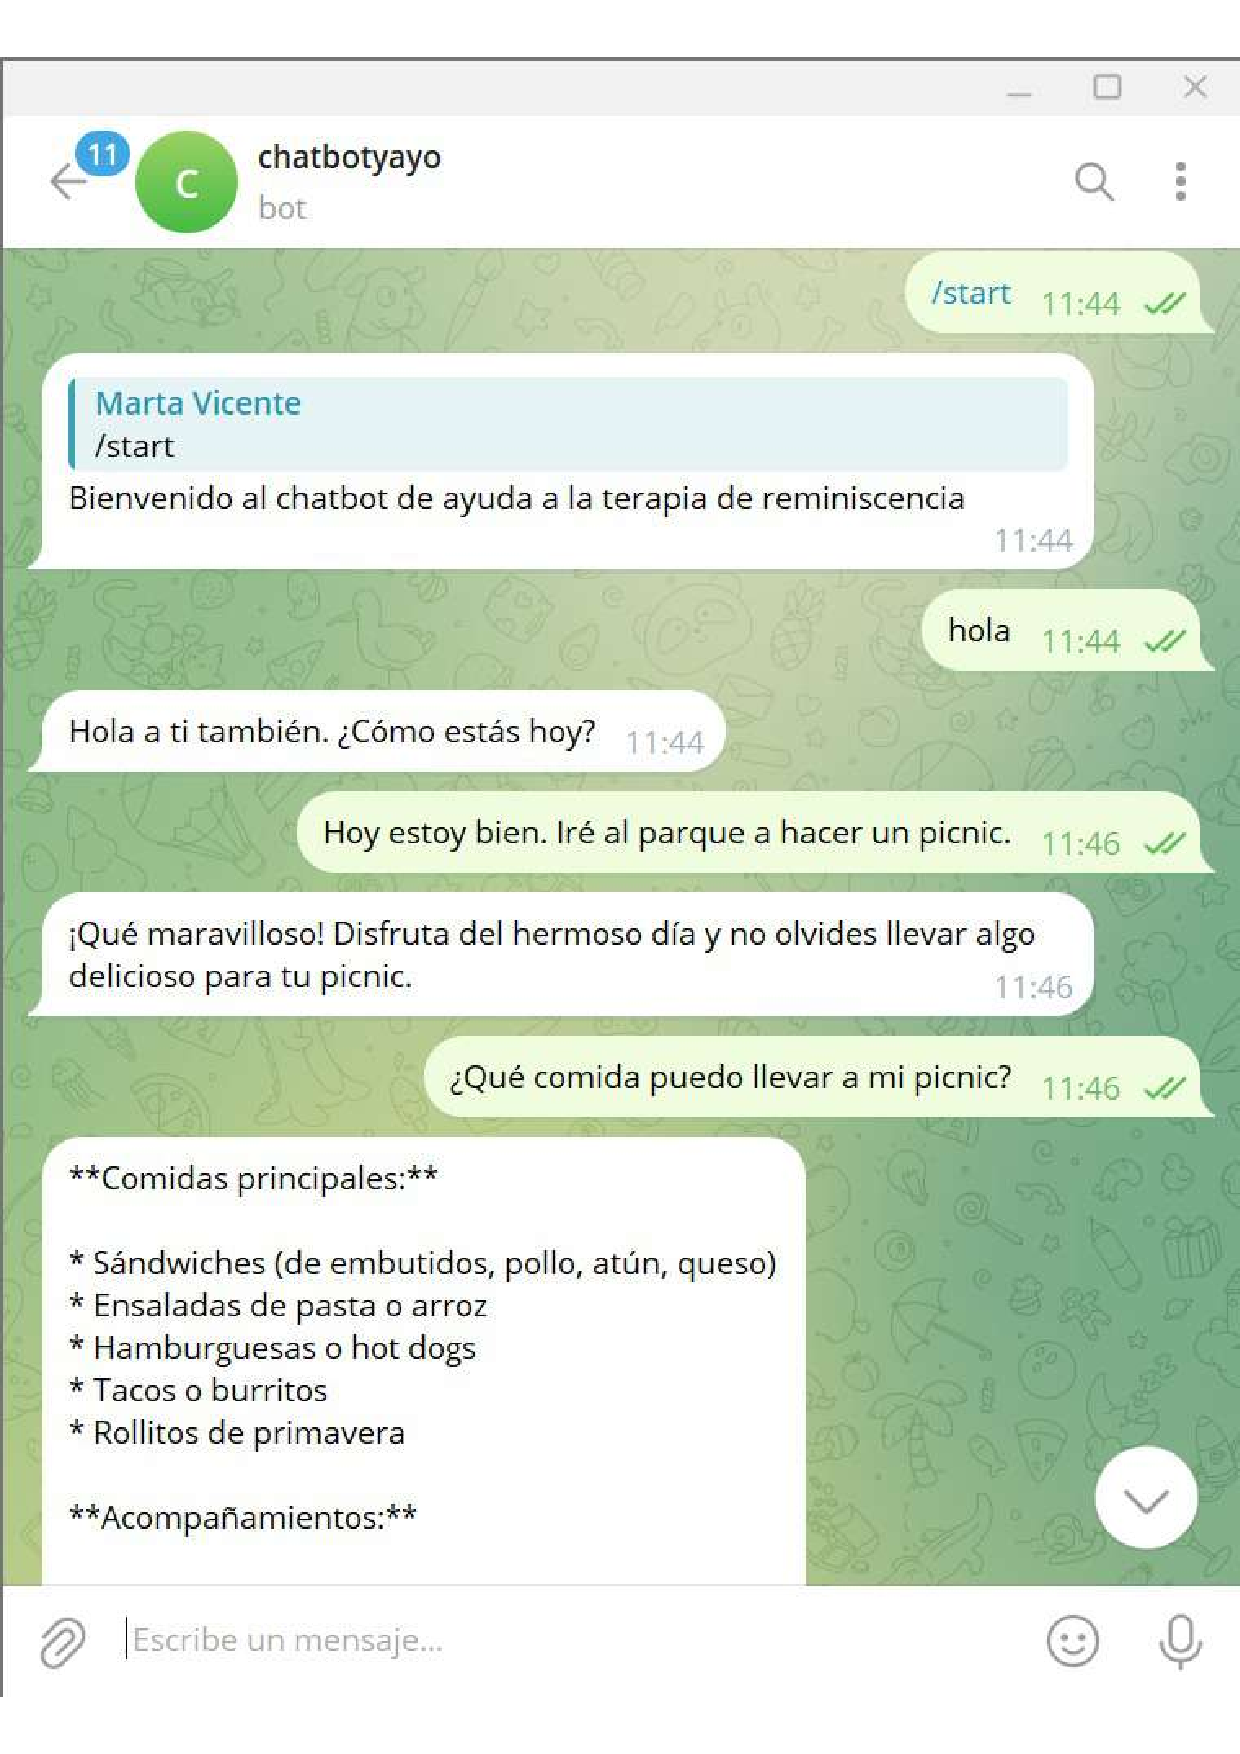
\includegraphics[width=0.5\textwidth]{Imagenes/telegram1}

%PRIMERA VERSIÓN EN BARD
%PRIMERA VERSIÓN EN GEMMA
%PRIMERA VERSIÓN GEMINI - GOOGLE COLLABORATE
%REFACTORIZACIÓN PARA HACER VERSIÓN LOCAL
%TELEGRAM
%GENERAR LAS ETAPAS 
%IMAGENES
%WHISPER
%GRÁFOS
%GENERACIÓN DE HISTORIAS DE VIDA
Para configurarlo, en primer lugar hay que ejecutar el programa mibot.py estando en telegram en la conversaa conversación de telegram el comando /start para comenzar la conversación y ya. 

Sin embago, y pese a las grandes funcionalidades de todas estas alternativas nos hemos decantado por hacer una interfaz con telegram desarrollando nuestro propio chatbot usando rasa. 

Para desarrollar el chatbot de telegram me he decantado por usar la interfaz de telegram para la cuál se necesita la API de Rasa. Las principales ventajas que ofrece esta herramienta es la facilidad del manejo de la interfaz pues telegram es una herramienta muy conocida con la que los terapeutas pueden estar más familiarizados. Además, esto nos permite también usar la versión del chatbotyayo para móvil. 

Para crear está interfaz hay que: 
1. Instalar rasa
2. Instalar telegram 
2. Obtener una api de rasa
4. crear un nuevo chatbot desde telegram con @botFather
5. Enviar a tu chatbot el comando /start

Una vez seguidos todos estos pasos ya puedes comenzar a interactuar con la API de rasa. 


\section{Respuestas de Gemini}

El modelo más apropiado para el procesamiento de texto es $gemini-pro$. La estructura de las respuestas de este modelo es la siguiente. 

\begin{lstlisting}[style=SpyderStyle, caption={Estructura de una respuesta de Gemini}, captionpos=b, label={lst:python},breaklines = true]
{
	"candidates": [
	{
		"content": {
			"parts": [
			{
				"text": string
			}
			]
		},
		"finishReason": enum (FinishReason),
		"safetyRatings": [
		{
			"category": enum (HarmCategory),
			"probability": enum (HarmProbability),
			"blocked": boolean
		}
		],
		"citationMetadata": {
			"citations": [
			{
				"startIndex": integer,
				"endIndex": integer,
				"uri": string,
				"title": string,
				"license": string,
				"publicationDate": {
					"year": integer,
					"month": integer,
					"day": integer
				}
			}
			]
		}
	}
	],
	"usageMetadata": {
		"promptTokenCount": integer,
		"candidatesTokenCount": integer,
		"totalTokenCount": integer
	}
}
\end{lstlisting}

\begin{itemize}
\item \textbf{text}	El texto generado.
\item \textbf{finishReason}	El motivo por el que el modelo dejó de generar tokens. Si está vacío, el modelo no dejó de generar los tokens. El motivo puede ser cualquiera de los siguientes:
\begin{enumerate}
	\item $FINISH\_REASON\_UNSPECIFIED$: no se especifica el motivo de finalización.
	\item $FINISH\_REASON\_STOP$: punto de detención natural del modelo o secuencia de detención proporcionada.
	\item $FINISH\_REASON\_MAX\_TOKENS$: se alcanzó la cantidad máxima de tokens especificada en la solicitud.
	\item $FINISH\_REASON\_SAFETY$: la generación del token se detuvo porque la respuesta se marcó por motivos de seguridad. Ten en cuenta que Candidate.content está vacío si los filtros de contenido bloquean el resultado.
	\item $FINISH\_REASON\_RECITATION$: la generación del token se detuvo porque la respuesta se marcó para citas no autorizadas.
	\item $FINISH\_REASON\_OTHER$: todos los demás motivos que detuvieron el token
\end{enumerate}

\item \textbf{category}	La categoría de seguridad para la que se configura un umbral. Los valores aceptables son los siguientes:
Haz clic para expandir las categorías de seguridad
\begin{enumerate}
	\item $HARM\_CATEGORY\_SEXUALLY\_EXPLICIT$
	\item $HARM\_CATEGORY\_HATE\_SPEECH$
	\item $HARM\_CATEGORY\_HARASSMENT$
	\item $HARM\_CATEGORY\_DANGEROUS\_CONTENT$
\end{enumerate}
\item \textbf{probability}	Los niveles de probabilidad de daños en el contenido.
\begin{enumerate}
	\item $HARM\_PROBABILITY\_UNSPECIFIED$
	\item $NEGLIGIBLE$
	\item $LOW$
	\item $MEDIUM$
	\item $HIGH$
\end{enumerate}
\item \textbf{blocked}	Una marca boolean asociada con un atributo de seguridad que indica si la entrada o salida del modelo se bloqueó. Si blocked es true, el campo errors en la respuesta contiene uno o más códigos de error. Si blocked es false, la respuesta no incluye el campo errors.
\item \textbf{startIndex}	Un número entero que especifica dónde comienza una cita en el contenido.
\item \textbf{endIndex}	Un número entero que especifica dónde termina una cita en content.
\item \textbf{url}	Es la URL de una fuente de cita. Los ejemplos de una fuente de URL pueden ser un sitio web de noticias o un repositorio de GitHub.
\item \textbf{title}	Es el título de una fuente de cita. Los ejemplos de títulos de origen pueden ser los de un artículo de noticias o un libro.
\item \textbf{license}	Es la licencia asociada con una cita.
\item \textbf{publicationDate}	La fecha en que se publicó una cita. Sus formatos válidos son YYYY, YYYY-MM y YYYY-MM-DD.
\item \textbf{promptTokenCount}	Cantidad de tokens en la solicitud.
\item \textbf{candidatesTokenCount}	Cantidad de tokens en las respuestas.
\item \textbf{totalTokenCount}	Cantidad de tokens en la solicitud y las respuestas.
\end{itemize}